\documentclass[10pt, margin=1mm]{standalone}
\usepackage{tikz}
\usetikzlibrary{arrows,decorations.pathmorphing,backgrounds,positioning,fit,petri,shapes}
\pgfdeclarelayer{bg}    % declare background layer
\pgfsetlayers{bg,main}  % set the order of the layers (main is the standard layer)
\usepackage{graphicx}
\usepackage{amsmath,amssymb,amsfonts}
\usepackage{fontawesome}

\definecolor{myblue}{RGB}{76,114,176}
\definecolor{myorange}{RGB}{221,132,82}

\usetikzlibrary{shapes.multipart}

\begin{document}
    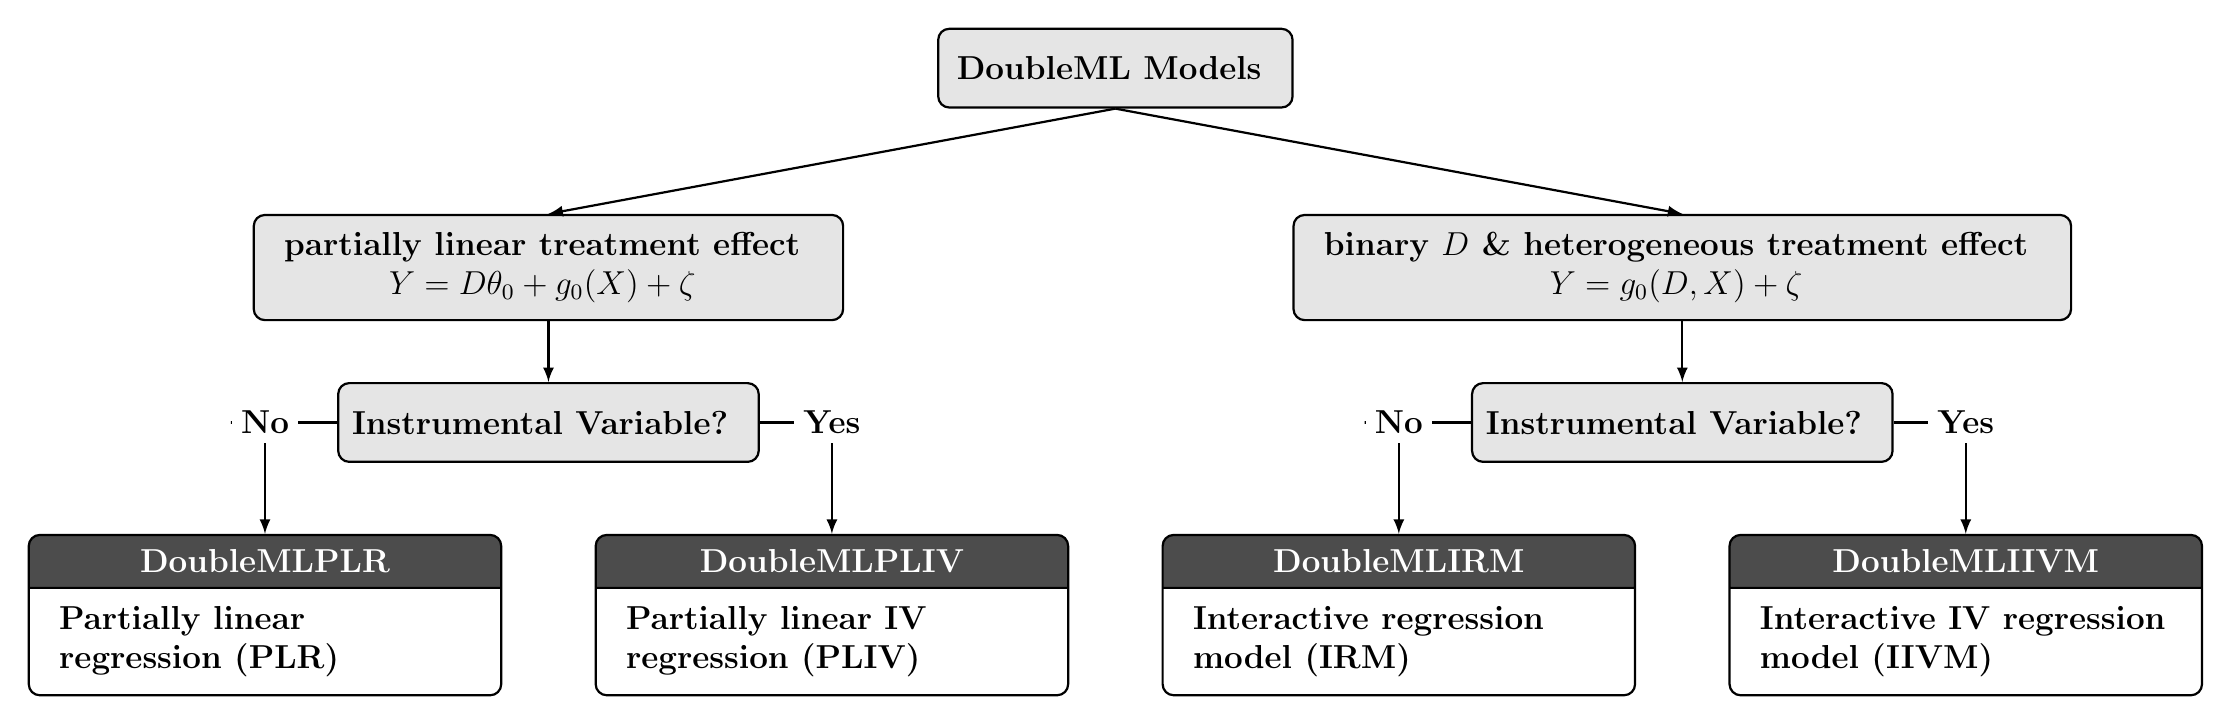
\begin{tikzpicture}[scale=0.9]
%[auto,scale=1,transition/.style={rectangle,draw=black!50,thick,
%inner sep=5pt,minimum width=8cm,minimum height=1cm,font=\large,text width=8cm}]
\tikzstyle{every node}=[font=\large\bf]



%\node[anchor=north, thick,above, fill=black!70, align=center,
%rectangle, inner sep=5pt, rounded corners, draw=black] at (0, 0) (s3) {
%\textcolor{white}{Data-Backend}
%};

\node[anchor=north, thick,above, fill=black!10, align=center,
minimum width=4.5cm, minimum height=1cm,
rectangle, inner sep=5pt, rounded corners, draw=black] at (0, 0) (model) {
DoubleML Models
};

\node[anchor=north, thick,above, fill=black!10, align=center,
minimum width=4.5cm, minimum height=1cm,
rectangle, inner sep=5pt, rounded corners, draw=black] at (-8, -3) (linear) {
\begin{tabular}{c}
partially linear treatment effect\\
$
Y = D \theta_0 + g_0(X) + \zeta
$
\end{tabular}
};

\node[anchor=north, thick,above, fill=black!10, align=center,
minimum width=4.5cm, minimum height=1cm,
rectangle, inner sep=5pt, rounded corners, draw=black] at (8, -3) (heterogeneous) {
\begin{tabular}{c}
binary $D$ \& heterogeneous treatment effect\\
$
Y = g_0(D, X) + \zeta
$
\end{tabular}
};


\node[anchor=north, thick,above, fill=black!10, align=center,
minimum width=4.5cm, minimum height=1cm,
rectangle, inner sep=5pt, rounded corners, draw=black] at (-8, -5) (l_iv) {
Instrumental Variable?
};

\node[anchor=north, thick,above, fill=black!10, align=center,
minimum width=4.5cm, minimum height=1cm,
rectangle, inner sep=5pt, rounded corners, draw=black] at (8, -5) (h_iv) {
Instrumental Variable?
};


\node[thick,below,
minimum width=6cm,
rectangle split,rectangle split parts=2, inner sep=5pt, rounded corners, draw=black,
rectangle split part align={center, left},
rectangle split part fill={black!70, white}] at (-12, -6) (plr) {
\textcolor{white}{
DoubleMLPLR}
\nodepart{two}{%
\begin{tabular}{l}
Partially linear \\
regression (PLR)
\end{tabular}}
};

\node[thick,below,
minimum width=6cm,
rectangle split,rectangle split parts=2, inner sep=5pt, rounded corners, draw=black,
rectangle split part align={center, left},
rectangle split part fill={black!70, white}] at (-4, -6) (pliv) {
\textcolor{white}{
DoubleMLPLIV}
\nodepart{two}{%
\begin{tabular}{l}
Partially linear IV \\
regression (PLIV)
\end{tabular}}
};

\node[thick,below,
minimum width=6cm,
rectangle split,rectangle split parts=2, inner sep=5pt, rounded corners, draw=black,
rectangle split part align={center, left},
rectangle split part fill={black!70, white}] at (4, -6) (irm) {
\textcolor{white}{
DoubleMLIRM}
\nodepart{two}{%
\begin{tabular}{l}
Interactive regression \\
model (IRM)
\end{tabular}}
};

\node[thick,below,
minimum width=6cm,
rectangle split,rectangle split parts=2, inner sep=5pt, rounded corners, draw=black,
rectangle split part align={center, left},
rectangle split part fill={black!70, white}] at (12, -6) (iivm) {
\textcolor{white}{
DoubleMLIIVM}
\nodepart{two}{%
\begin{tabular}{l}
Interactive IV regression \\
model (IIVM)
\end{tabular}}
};


\draw[-latex, thick] (model.south) -- (linear.north);
\draw[-latex, thick] (model.south) -- (heterogeneous.north);

\draw[-latex, thick] (linear.south) -- (l_iv.north);
\draw[-latex, thick] (heterogeneous.south) -- (h_iv.north);

\draw[-latex, thick] (l_iv.west) -- ++(-1.5, 0) -| node[midway,fill=white] {No} (plr.north);
\draw[-latex, thick] (l_iv.east) -- ++(1.5, 0) -| node[midway,fill=white] {Yes} (pliv.north);
\draw[-latex, thick] (h_iv.west) -- ++(-1.5, 0) -| node[midway,fill=white] {No} (irm.north);
\draw[-latex, thick] (h_iv.east) -- ++(1.5, 0) -| node[midway,fill=white] {Yes} (iivm.north);


\end{tikzpicture}

\end{document}
